\documentclass[cal1spr16Lectures.tex]{subfiles}
%\AtBeginSubsection{
%	\begin{frame}[allowframebreaks]{}
%	\begin{multicols}{2}
%	\tableofcontents[currentsubsection]
%	\end{multicols}
%	\end{frame}
%	}
	
\begin{document}

%\section[Week 3]{Week 3: 1-5 February}

% % %
\subsubsection{\bf Friday 5 February}
\begin{frame}[allowframebreaks]{Fri 5 Feb}
\begin{itemize}%\footnotesize
\item GET YOUR CLICKER NOW.  If you haven't gotten any email from me, then your clicker should be working fine.  	
\item EXAM 1 is one week from today.  Covers up to \S 3.1 (see the semester schedule of material on the course webpage).  \alert{You must attend your own lecture on exam day.}  CEA: Register with the CEA office for a time on 12 Feb, as close to your normal lecture time as possible.
\item Look at old Wheeler exams to study.
\url{comp.uark.edu/~ashleykw}
\end{itemize}
\end{frame}

% % %
\begin{frame}
\begin{exe} Which of the following functions is continuous for all real values of $x$?
\begin{itemize}
\item[(A)\;] $f(x)=\frac{x^2}{2x+1}$
\item[(B)\;] $g(x)=\sqrt{3x^2-2}$
\item[(C)\;] $h(x)=\frac{5x}{|x^8-1|}$
\item[(D)\;] $j(x)=\frac{5x}{x^8+1}$
\end{itemize}
\end{exe}
\end{frame}

% % %
\subsubsection{Book Problems}
\begin{frame}
\begin{block}{2.6 Book Problems} 9-25 (odds), 35-45 (odds), 59, 61, 63, 83, 85 \end{block} 
\end{frame}

% % %
\subsection[2.7 Precise Definitions of Limits]{\S 2.7 Precise Definitions of Limits}
% % %

% % %
\begin{frame}{\S 2.7 Precise Definitions of Limits}\small
So far in our dealings with limits, we have used informal terms such as ``sufficiently close" and ``arbitrarily large".  Now we will formalize what these terms mean mathematically.

\vspace{1pc}
\textbf{Recall:} $|f(x)-L|$ and $|x-a|$ refer to the distances between $f(x)$ and $L$ and between $x$ and $a$.

\vspace{1pc}
Also, recall that when we worked informally with limits, we wanted $x$ to approach $a$, \alert{but not necessarily equal $a$}.  Likewise, we wanted $f$ to get arbitrarily close to $L$, but not necessarily equal $L$.
\end{frame}

% % %
\begin{frame}\footnotesize
\begin{dfn}
Assume that $f(x)$ exists for all $x$ in some open interval (open means: neither of the endpoints not included) containing $a$, except possibly at $a$.  \textbf{``The limit of $f(x)$ as $x$ approaches $a$ is $L$"}, i.e.,
\[\lim_{x \to a}f(x)=L,\]
means \textbf{for any $\epsilon > 0$ there exists $\delta > 0$ such that} 
\[|f(x)-L|<\epsilon \quad \textbf{whenever} \quad 0<|x-a|<\delta.\]
\end{dfn}
\begin{que}
Why $0<|x-a|$ but not for $|f(x)-L|$?
\end{que}

\end{frame}

% % %
\subsubsection{$\epsilon$ and $\delta$}
% % %

% % %
\begin{frame}{\small $\epsilon$ and $\delta$}\small
When we worked informally with limits, we saw $f(x)$ get closer and closer to $L$ as $x$ got closer and closer to $a$. 

\begin{que} If we want the distance between $f(x)$ and $L$ to be less than $1$, how close does $x$ have to be to $a$? What if we want $|f(x)-L|<0.5$?  $0.5$? $0.1$? $0.01$?  
\end{que}
\end{frame}

% % %
\subsubsection{Seeing $\epsilon$s and $\delta$s on a Graph}
% % %

% % %
\begin{frame}{\small Seeing $\epsilon$s and $\delta$s on a Graph}\footnotesize
\begin{ex}
\begin{columns}[T]
	\begin{column}{.36\textwidth}
		\centering{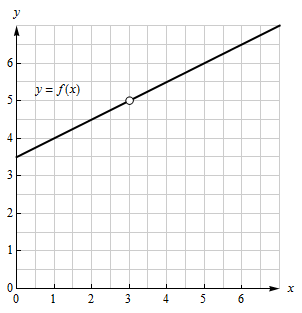
\includegraphics[scale=0.55]{pictures/Fig2_57}}
	\end{column}
	\begin{column}{.5\textwidth}
		Using the graph, for each $\epsilon >0$, determine a value of $\delta>0$ to satisfy the statement 
		\begin{multline*}|f(x)-5|<\epsilon\quad\text{whenever} \\
			0<|x-3|<\delta.\end{multline*}  
		\vspace{-1.5pc}
		\begin{itemize}
		\item[(a) ] $\epsilon=1$ 
		\item[(b) ] $\epsilon=0.5$.
		\end{itemize}
	\end{column}
\end{columns}
\end{ex}
\end{frame} 

% % %
\begin{frame}{\small Seeing $\epsilon$s and $\delta$s on a Graph, cont.}\footnotesize
When $\epsilon=1$:
\vspace{-0.25pc}
\begin{columns}
\begin{column}{.36\textwidth}
\begin{block}
\centering{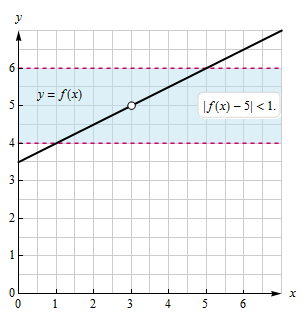
\includegraphics[scale=0.45]{pictures/Fig2_57a}}
\end{block}
\end{column}
\begin{column}{.36\textwidth}
\begin{block}
\centering{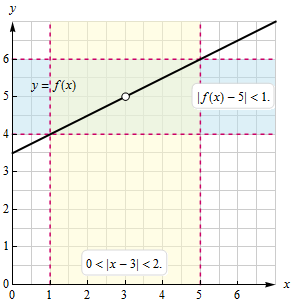
\includegraphics[scale=0.47]{pictures/Fig2_57b}}
\end{block}
\end{column}
\end{columns}
\vspace{-0.75pc}
\flushright $\dots\;\delta=2$
\end{frame}

% % %
\begin{frame}{\small Seeing $\epsilon$s and $\delta$s on a Graph, cont.}\footnotesize
When $\epsilon=0.5$:
\vspace{-0.25pc}
\begin{columns}
\begin{column}{.36\textwidth}
\begin{block}
\centering{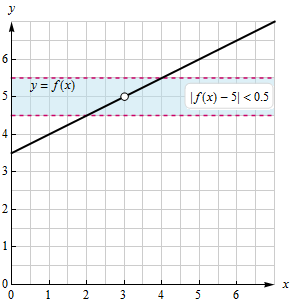
\includegraphics[scale=0.47]{pictures/Fig2_58}}
\end{block}
\end{column}
\begin{column}{.36\textwidth}
\begin{block}
\centering{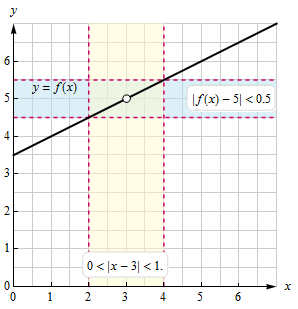
\includegraphics[scale=0.47]{pictures/Fig2_58a}}
\end{block}
\end{column}
\end{columns}
\vspace{-0.75pc}
\flushright $\dots\;\delta=1$
\end{frame}

% % %
\begin{frame}{}
The $\epsilon$s and $\delta$s give a way to visualize computing the limit, and prove it exists.  As the $\epsilon$s get smaller and smaller, we want there to always be a $\delta$.  In this example,
\[\lim_{x\to 3}f(x)=5.\]
\end{frame}

% % %
\begin{frame}\footnotesize
\begin{exe}
\vspace{0.75pc}
\begin{columns}[T]
	\begin{column}{.22\textwidth}
		\centering{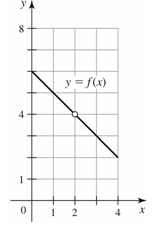
\includegraphics[scale=0.85]{pictures/Ch2Sect7_Exer10}}
	\end{column}
	\begin{column}{.6\textwidth}
		Using the graph, for each $\epsilon>0$, determine a value of $\delta>0$ to satisfy the statement
		\begin{multline*}|f(x)-4|<\epsilon\quad\text{whenever} \\
			0<|x-2|<\delta.\end{multline*}  
		\vspace{-1pc}
		\begin{itemize}
		\item[(a) ] $\epsilon=1$ 
		\item[(b) ] $\epsilon=0.5$.
		\end{itemize}
	\end{column}
\end{columns}
\end{exe}
\end{frame} 

% % %
\subsubsection{Finding a Symmetric Interval}
% % % 

% % %
\begin{frame}{\small Finding a Symmetric Interval}
\begin{que}When finding an interval $(a-\delta, a+\delta)$ around the point $a$, what happens if you compute two different $\delta$s?\end{que}  
{\bf Answer:}  To obtain a symmetric interval around $a$, use the smaller of the two $\delta$s as your distance around $a$.
\end{frame}

% % %
\begin{frame}\footnotesize
\begin{exe}
\vspace{0.75pc}
\begin{columns}[T]
	\begin{column}{.4\textwidth}
		\centering{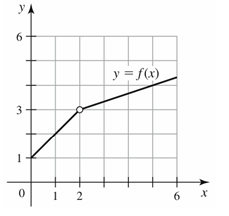
\includegraphics[scale=0.9]{pictures/Ch2Sect7_Exer15}}
	\end{column}
	\begin{column}{.55\textwidth}
		The graph of $f(x)$ shows 
		\[\lim_{x \to 2}f(x)=3.\] 
		For $\epsilon=1$, find the corresponding value of $\delta>0$ so that
		\begin{multline*}|f(x)-3|<\epsilon\quad\text{whenever} \\
			0<|x-2|<\delta.\end{multline*}  
	\end{column}
\end{columns}
\end{exe}
\end{frame}

\end{document}